% Boundary layer of width delta ~ eps along the outer boundary (affine-BC problem of Eq. Kapp).
% Compile: pdflatex boundary_layer.tex  ->  boundary_layer.pdf  (copied to ../boundary_layer.pdf)
\documentclass[tikz,border=3pt]{standalone}
\usepackage{amsmath,amssymb}
\usetikzlibrary{arrows.meta,decorations.pathreplacing}
% Shared colours and line styles of the boundary-condition diagrams.
\definecolor{dir}{HTML}{B03A2E}       % Dirichlet (imposed temperature)
\definecolor{neu}{HTML}{1F4E79}       % Neumann (insulated)
\definecolor{per}{HTML}{1E8449}       % periodic
\definecolor{solidfill}{HTML}{E9EEF3} % solid material
\definecolor{homfill}{HTML}{D6E4F0}   % homogenized material
\definecolor{layer}{HTML}{F0B27A}     % boundary layer
\tikzset{insul/.style={densely dashed}}

\newcommand{\hole}[2]{%
  \begin{scope}[shift={(#1,#2)}, rotate=40]
    \fill[white] (0,0) ellipse (0.3*0.8 and 0.12*0.8);
    \draw[neu, insul] (0,0) ellipse (0.3*0.8 and 0.12*0.8);
  \end{scope}}
\begin{document}
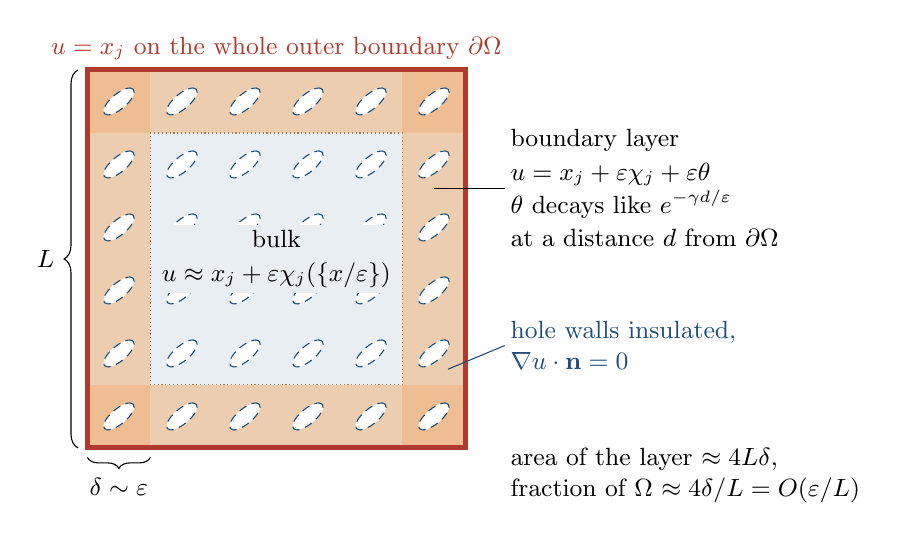
\begin{tikzpicture}[font=\small]
  % plate of 6 x 6 cells of size eps = 0.8, L = 4.8
  \fill[solidfill] (0,0) rectangle (4.8,4.8);
  \begin{scope}
    \clip (0,0) rectangle (4.8,4.8);
    \fill[layer, fill opacity=0.55] (0,0) rectangle (0.8,4.8);
    \fill[layer, fill opacity=0.55] (4.0,0) rectangle (4.8,4.8);
    \fill[layer, fill opacity=0.55] (0,0) rectangle (4.8,0.8);
    \fill[layer, fill opacity=0.55] (0,4.0) rectangle (4.8,4.8);
  \end{scope}
  \draw[layer!70!black, densely dotted] (0.8,0.8) rectangle (4.0,4.0);
  \foreach \i in {0,...,5}{\foreach \j in {0,...,5}{\hole{0.4+0.8*\i}{0.4+0.8*\j}}}
  \draw[dir, line width=1.8pt] (0,0) rectangle (4.8,4.8);
  % labels
  \node[dir, above] at (2.4,4.8) {$u=x_j$ on the whole outer boundary $\partial\Omega$};
  \node[align=center, fill=solidfill, inner sep=2pt] at (2.4,2.4)
     {bulk\\[1pt] $u\approx x_j+\varepsilon\chi_j(\{x/\varepsilon\})$};
  % layer thickness
  \draw[decorate, decoration={brace, amplitude=4pt, mirror}] (0,-0.12) -- (0.8,-0.12)
     node[midway, below=4pt] {$\delta\sim\varepsilon$};
  \draw[decorate, decoration={brace, amplitude=5pt}] (-0.12,0) -- (-0.12,4.8)
     node[midway, left=5pt] {$L$};
  % callouts on the right
  \draw[thin] (4.4,3.3) -- (5.3,3.3);
  \node[right, align=left] at (5.25,3.3)
     {boundary layer\\[1pt] $u=x_j+\varepsilon\chi_j+\varepsilon\theta$\\[1pt]
      $\theta$ decays like $e^{-\gamma d/\varepsilon}$\\[1pt] at a distance $d$ from $\partial\Omega$};
  \draw[neu, thin] (4.4+0.18,1.2-0.2) -- (5.3,1.3);
  \node[neu, right, align=left] at (5.25,1.3) {hole walls insulated,\\ $\nabla u\cdot\mathbf{n}=0$};
  \node[right, align=left] at (5.25,-0.35)
     {area of the layer $\approx 4L\delta$,\\ fraction of $\Omega$ $\approx 4\delta/L=O(\varepsilon/L)$};
\end{tikzpicture}
\end{document}
